\documentclass[12pt]{article}
\setlength{\oddsidemargin}{0in}
\setlength{\evensidemargin}{0in}
\setlength{\textwidth}{6.5in}
\setlength{\parindent}{0in}
\setlength{\parskip}{\baselineskip}

\usepackage{amsmath,amsfonts,amssymb,graphicx}

%\title{Review of Newtonian Mechanics}

\begin{document}

PHYS 374 Fall 2020\hfill Worksheet 4: Revenge of the Frictionless Ramp\\
\\
Name: \\
\\
Please submit as a PDF on Moodle. Include any calculations made using external tools.

\hrulefill
\\
\\
Let's revisit the mass on a frictionless ramp using calculus of variations. We are interested in the motion of the block down the ramp, as well as the motion of the ramp itself. \begin{figure}[h]
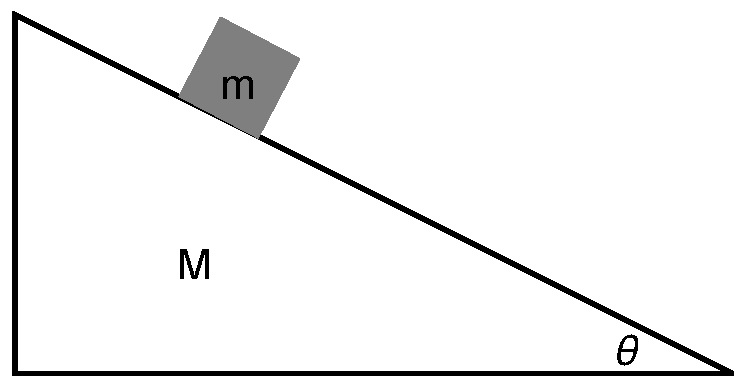
\includegraphics[width=5cm]{Diagram.pdf}
\centering
\end{figure}
\begin{enumerate}
\item Write down expressions for the position of the ramp and the position of the block. Make sure to use no more variables than the system has degrees of freedom.
\item What are the kinetic and potential energies associated with the ramp? Is there a more convenient reference point?
\item What are the kinetic and potential energies associated with the block? Is there a more convenient reference point?
\item Write down the Lagrangian of the system. Double check your signs!
\item Use the Euler-Lagrange equations to find the equations of motion.
\item Solve the equations to find the acceleration of the ramp and the acceleration of block along the surface of the ramp.
\item Does this system behave as expected when $M$ and/or $\theta$ take extreme values?
\item How does the Lagrangian solution compare to our earlier Newtonian solution for the same system?
\end{enumerate}
\end{document}